\documentclass{article}

\usepackage[preprint]{neurips_2026}

\usepackage[utf8]{inputenc}
\usepackage[T1]{fontenc}
\usepackage{hyperref}
\usepackage{url}
\usepackage{booktabs}
\usepackage{amsfonts}
\usepackage{amsmath}
\usepackage{nicefrac}
\usepackage{microtype}
\usepackage{xcolor}
\usepackage{graphicx}
\usepackage{float}
\usepackage{caption}

\title{Hybrid Unsupervised Risk Phenotyping and Supervised Classification for Breast Cancer Diagnosis}

\author{%
  Daniyal Siddiqui \\
  Department of Computer Science \\
  Rutgers University \\
  New Brunswick, NJ 08901 \\
  \texttt{dfs107@scarletmail.rutgers.edu} \\
  \And
  Samarth Suresh Shastry \\
  Department of Computer Science \\
  Rutgers University \\
  New Brunswick, NJ 08901 \\
  \texttt{ss5057@scarletmail.rutgers.edu} \\
}

\begin{document}

\maketitle

\begin{abstract}
Early identification of malignant breast masses is a high-impact classification problem because diagnostic decisions require
both predictive accuracy and interpretability. This project studies whether unsupervised morphology-based phenotypes can
support binary diagnosis prediction on the Wisconsin Diagnostic Breast Cancer dataset. We compare a majority-class dummy
model, logistic regression, random forest, and radial basis function support vector machine against a proposed hybrid pipeline
that first learns K-Means phenotypes from standardized cell-nuclei measurements and then appends one-hot cluster indicators
to a logistic regression classifier. All preprocessing, scaling, clustering, and encoding steps are fit only on the training set to
reduce leakage. On a stratified 20\% held-out test set, the best accuracy is achieved by the RBF SVM at 98.25\%, while the
random forest obtains the strongest ROC-AUC at 0.9970. The hybrid K-Means + Logistic model achieves 96.49\% accuracy
and 0.9927 ROC-AUC. The hybrid model does not outperform the strongest supervised baselines, but it provides a transparent
phenotype layer that helps explain the structure of the feature space and supports clinically readable error analysis. These
results suggest that unsupervised phenotyping can be useful for interpretability, but the WDBC dataset is already highly
separable using standard supervised models.
\end{abstract}

\section{Introduction}

Breast cancer diagnosis often depends on distinguishing benign from malignant tissue using measurements derived from
medical imaging or biopsy procedures. From a data science perspective, this is a binary classification problem where false
negatives are especially costly because a malignant case predicted as benign can delay treatment. A useful model should
therefore achieve strong recall for malignant cases while remaining interpretable enough for human review.

This project asks the following research question: Can unsupervised morphology-based risk phenotypes learned with
K-Means improve or explain supervised prediction of malignant versus benign breast masses? The project uses the Wisconsin
Diagnostic Breast Cancer (WDBC) dataset, which contains 569 samples and 30 real-valued features computed from digitized
fine needle aspirate images of breast masses \cite{uci_wdbc}. These features describe nucleus size, shape, texture, concavity, and related
morphology measurements.

The main contributions are threefold. First, we build a leakage-aware preprocessing pipeline that remaps the binary
diagnosis target, standardizes numeric predictors, learns K-Means clusters only on training data, and one-hot encodes cluster
membership before supervised training. Second, we compare the proposed hybrid model against multiple baselines using
accuracy, precision, recall, F1, ROC-AUC, average precision, and confusion-matrix error analysis. Third, we provide PCA
visualizations and permutation feature importance to connect predictive results with interpretable morphology patterns.

\section{Related Work}

\paragraph{Breast cancer diagnosis with machine learning.} The WDBC dataset is widely used as a benchmark for supervised
diagnosis because its features are quantitative measurements extracted from breast-mass cell nuclei \cite{uci_wdbc}. Prior work has
applied supervised classifiers such as multilayer perceptrons, support vector machines, random forests, and feature-selection
pipelines to this dataset, often reporting high performance because malignant and benign cases are strongly separable in
several morphology dimensions \cite{aamir2022predicting}.

\paragraph{Supervised classification baselines.} Logistic regression is a strong linear baseline for binary classification because it
estimates class probabilities through a regularized logit model. Random forests combine many decision trees trained with
randomized feature and sample variation, reducing variance and capturing nonlinear interactions \cite{breiman2001random}. Support vector machines
maximize a separating margin and, with a radial basis function kernel, can model nonlinear class boundaries \cite{cortes1995support}. These
models are appropriate baselines because they represent increasing levels of complexity: linear, tree ensemble, and nonlinear
margin-based classification.

\paragraph{Unsupervised phenotyping and visualization.} K-Means clusters data by minimizing within-cluster squared distances
around $k$ centroids \cite{macqueen1967kmeans}. In this project, K-Means is not used as the final classifier. Instead, it creates a morphology phenotype
variable that is one-hot encoded and added to the supervised model. PCA is used only for visualization by projecting
standardized 30-dimensional data into two principal components that explain the largest variance directions \cite{hotelling1933analysis}. The
implementation uses scikit-learn, a standard Python machine learning library \cite{pedregosa2011scikit}.

\section{Methodology}

\subsection{Dataset and Target Definition}

The dataset contains 569 patient-level samples, 30 numeric predictors, and a binary diagnosis label. The original scikit-learn
target uses 0 for malignant and 1 for benign, so we remap it to a more natural modeling target:
\[
y_i = \begin{cases}
1, & \text{if diagnosis is malignant,} \\
0, & \text{if diagnosis is benign.}
\end{cases}
\]
This makes malignant diagnosis the positive class for precision, recall, F1, ROC-AUC, and average precision. The class
distribution is 212 malignant samples and 357 benign samples. We use an 80/20 stratified train/test split with random seed 42,
producing 455 training samples and 114 held-out test samples.

\subsection{Preprocessing and Leakage Prevention}

The preprocessing design follows a strict train/test separation. The split is performed before scaling, clustering, encoding, or
model fitting. The main numeric features are standardized with $z = (x-\mu)/\sigma$, where $\mu$ and $\sigma$ are learned from the training set
only and then applied to the test set. This is important because K-Means and regularized logistic regression are scale-sensitive.

The raw dataset does not contain source categorical predictors. To satisfy the project requirement for categorical processing
in a meaningful way, We create a derived categorical variable using K-Means cluster membership. The number of clusters is
selected using training-only silhouette score over $k \in \{2, 3, 4, 5, 6\}$. The selected model uses $k = 2$. The learned cluster labels
are categorical phenotype IDs, so they are transformed using one-hot encoding. If $c_i \in \{1, \ldots, k\}$ is the cluster assignment
for sample $i$, the encoder produces a vector $e(c_i)$ whose entries indicate cluster membership. The final hybrid feature vector is
\[
z_i^{\text{hybrid}} = [\text{StandardScaler}(x_i), e(c_i)].
\]
The one-hot encoder is fit on training cluster labels only. Test samples receive cluster labels through the training-fitted
K-Means model and are then encoded through the training-fitted encoder.

\subsection{Models}

We compare five models:
\begin{enumerate}
    \item \textbf{Majority Dummy}: predicts the most frequent class and acts as a lower-bound baseline.
    \item \textbf{Logistic Regression}: standardized predictors with class-balanced logistic regression.
    \item \textbf{Random Forest}: 100-tree class-balanced random forest.
    \item \textbf{RBF SVM}: standardized predictors with a radial basis function support vector machine.
    \item \textbf{Hybrid K-Means + Logistic}: standardized predictors plus one-hot encoded K-Means phenotype indicators, followed
    by class-balanced logistic regression.
\end{enumerate}
The hybrid model is the proposed pipeline. It tests whether a compact unsupervised representation of morphology groups adds
useful predictive or interpretive information beyond raw standardized measurements.

\subsection{Evaluation Metrics}

The primary metrics are accuracy, precision, recall, F1, ROC-AUC, and average precision. Recall is emphasized because
malignant false negatives are the most concerning error type. ROC-AUC evaluates ranking quality over all thresholds, while
average precision is useful because the positive class is smaller than the benign class. We also report confusion matrices
and permutation importance. Permutation importance measures how much ROC-AUC decreases when a feature is randomly
shuffled, which helps identify influential morphology measurements.

\section{Experiments and Results}

\subsection{K-Means Model Selection}

K-Means was selected using silhouette score on the training data only. Table~\ref{tab:kmeans} shows that $k = 2$ produced the highest
silhouette score, which is also intuitive for a dataset with two diagnostic outcomes. This does not mean that the clusters are
equivalent to diagnosis labels; rather, it suggests that a two-phenotype morphology partition is the most stable among the
tested values.

\begin{table}[H]
\centering
\caption{Training-only K-Means model selection.}
\label{tab:kmeans}
\begin{tabular}{ccc}
\toprule
$k$ & Silhouette score & Inertia \\
\midrule
2 & 0.3432 & 9254.8273 \\
3 & 0.3233 & 8075.3173 \\
4 & 0.2782 & 7344.3357 \\
5 & 0.1565 & 6810.1568 \\
6 & 0.1604 & 6328.7294 \\
\bottomrule
\end{tabular}
\end{table}

\begin{figure}[H]
\centering
\begin{minipage}{0.48\linewidth}
\centering
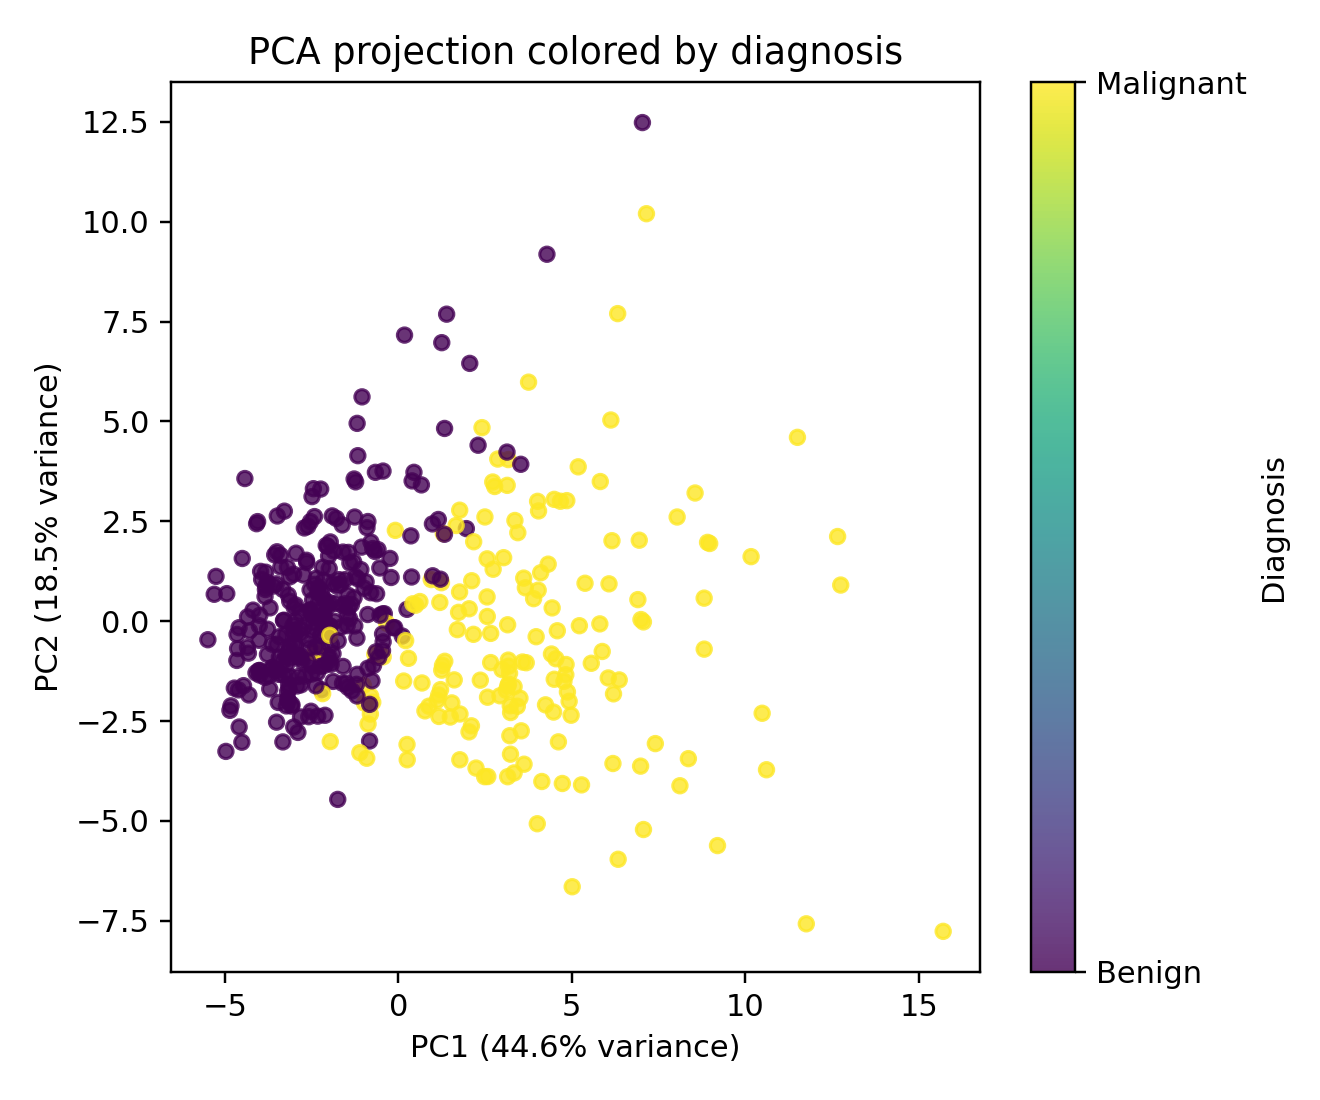
\includegraphics[width=\linewidth]{../outputs/figures/pca_diagnosis.png}
\caption*{(a) PCA colored by diagnosis.}
\end{minipage}
\hfill
\begin{minipage}{0.48\linewidth}
\centering
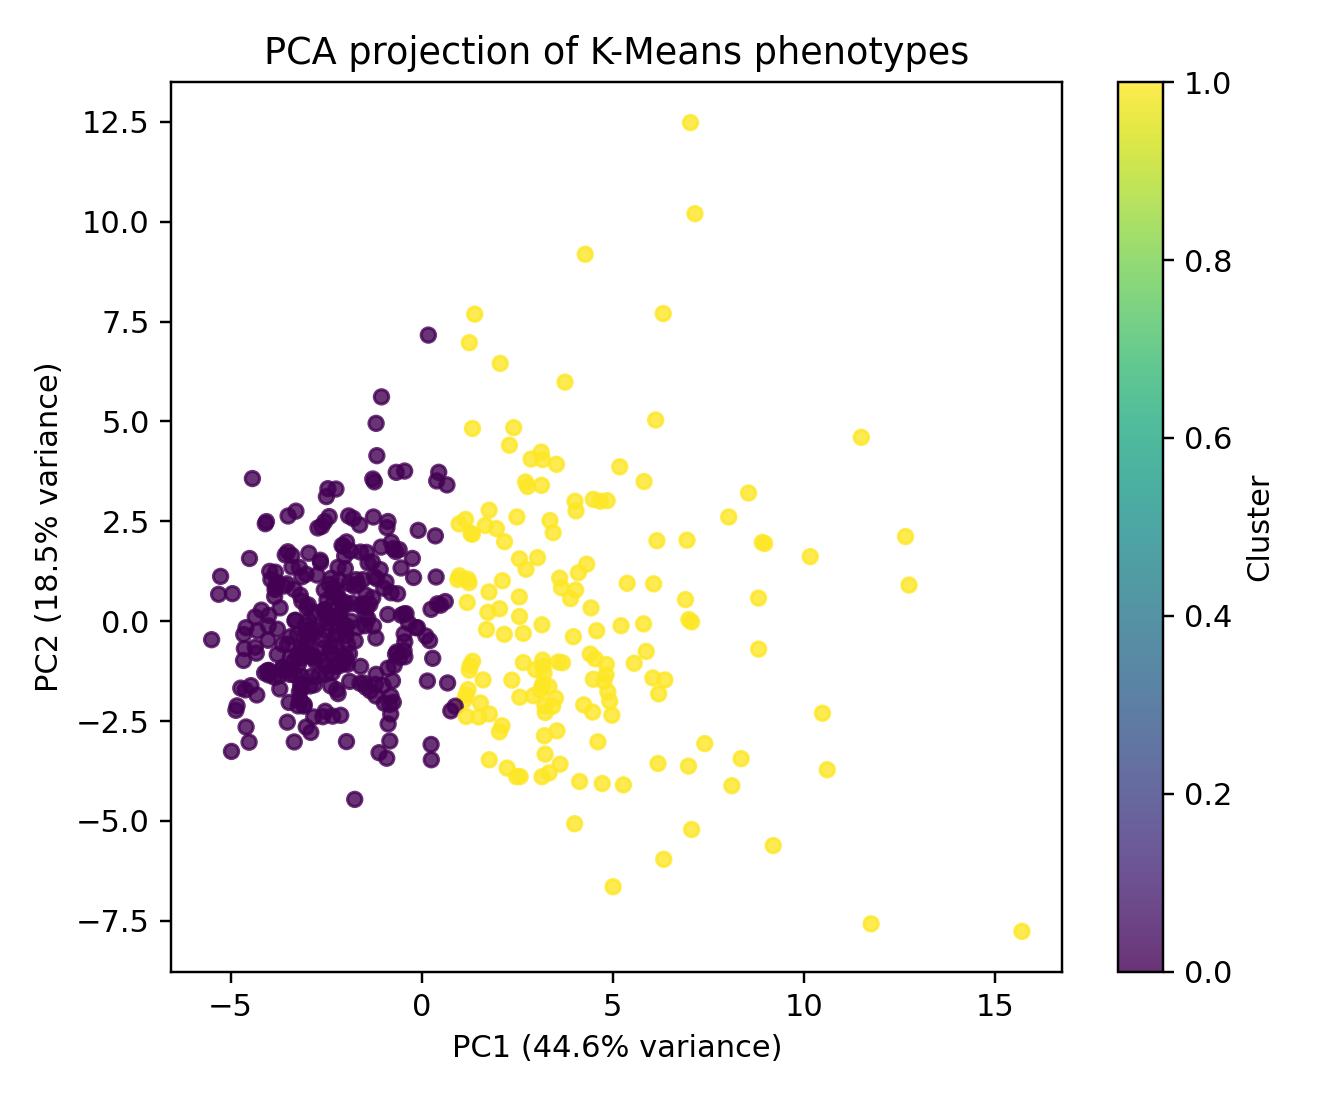
\includegraphics[width=\linewidth]{../outputs/figures/pca_kmeans_clusters.png}
\caption*{(b) PCA colored by K-Means phenotype.}
\end{minipage}
\caption{PCA projections show that the data contains a strong morphology gradient. The K-Means phenotypes broadly follow
the same geometry as the diagnostic separation, which supports their use as an interpretable derived categorical feature.}
\label{fig:pca}
\end{figure}

\subsection{Held-Out Test Performance}

Table~\ref{tab:testmetrics} reports performance on the 114-sample held-out test set. The RBF SVM achieves the highest accuracy, 98.25\%, with
only two malignant false negatives and no false positives. The random forest achieves the highest ROC-AUC, 0.9970, and
perfect precision at the default threshold, but it misses three malignant cases. Logistic regression is also strong, with 97.37\%
accuracy and 0.9954 ROC-AUC.

The proposed hybrid model achieves 96.49\% accuracy, 92.86\% recall, 95.12\% F1, and 0.9927 ROC-AUC. It is competitive,
but it does not outperform the strongest supervised models. This result is useful because it shows that the K-Means phenotype
variable preserves much of the diagnostic signal but does not add enough extra information to beat the direct nonlinear
baselines.

\begin{table}[H]
\centering
\caption{Held-out test metrics. Positive class is malignant.}
\label{tab:testmetrics}
\resizebox{\linewidth}{!}{%
\begin{tabular}{lcccccccccc}
\toprule
Model & Acc. & Prec. & Recall & F1 & ROC-AUC & Avg. Prec. & TN & FP & FN & TP \\
\midrule
Random Forest              & 0.9737 & 1.0000 & 0.9286 & 0.9630 & 0.9970 & 0.9952 & 72 & 0 & 3  & 39 \\
Logistic Regression        & 0.9737 & 0.9756 & 0.9524 & 0.9639 & 0.9954 & 0.9931 & 71 & 1 & 2  & 40 \\
RBF SVM                    & 0.9825 & 1.0000 & 0.9524 & 0.9756 & 0.9950 & 0.9937 & 72 & 0 & 2  & 40 \\
Hybrid K-Means + Logistic  & 0.9649 & 0.9750 & 0.9286 & 0.9512 & 0.9927 & 0.9896 & 71 & 1 & 3  & 39 \\
Majority Dummy             & 0.6316 & 0.0000 & 0.0000 & 0.0000 & 0.5000 & 0.3684 & 72 & 0 & 42 & 0  \\
\bottomrule
\end{tabular}%
}
\end{table}

\begin{figure}[H]
\centering
\begin{minipage}{0.48\linewidth}
\centering
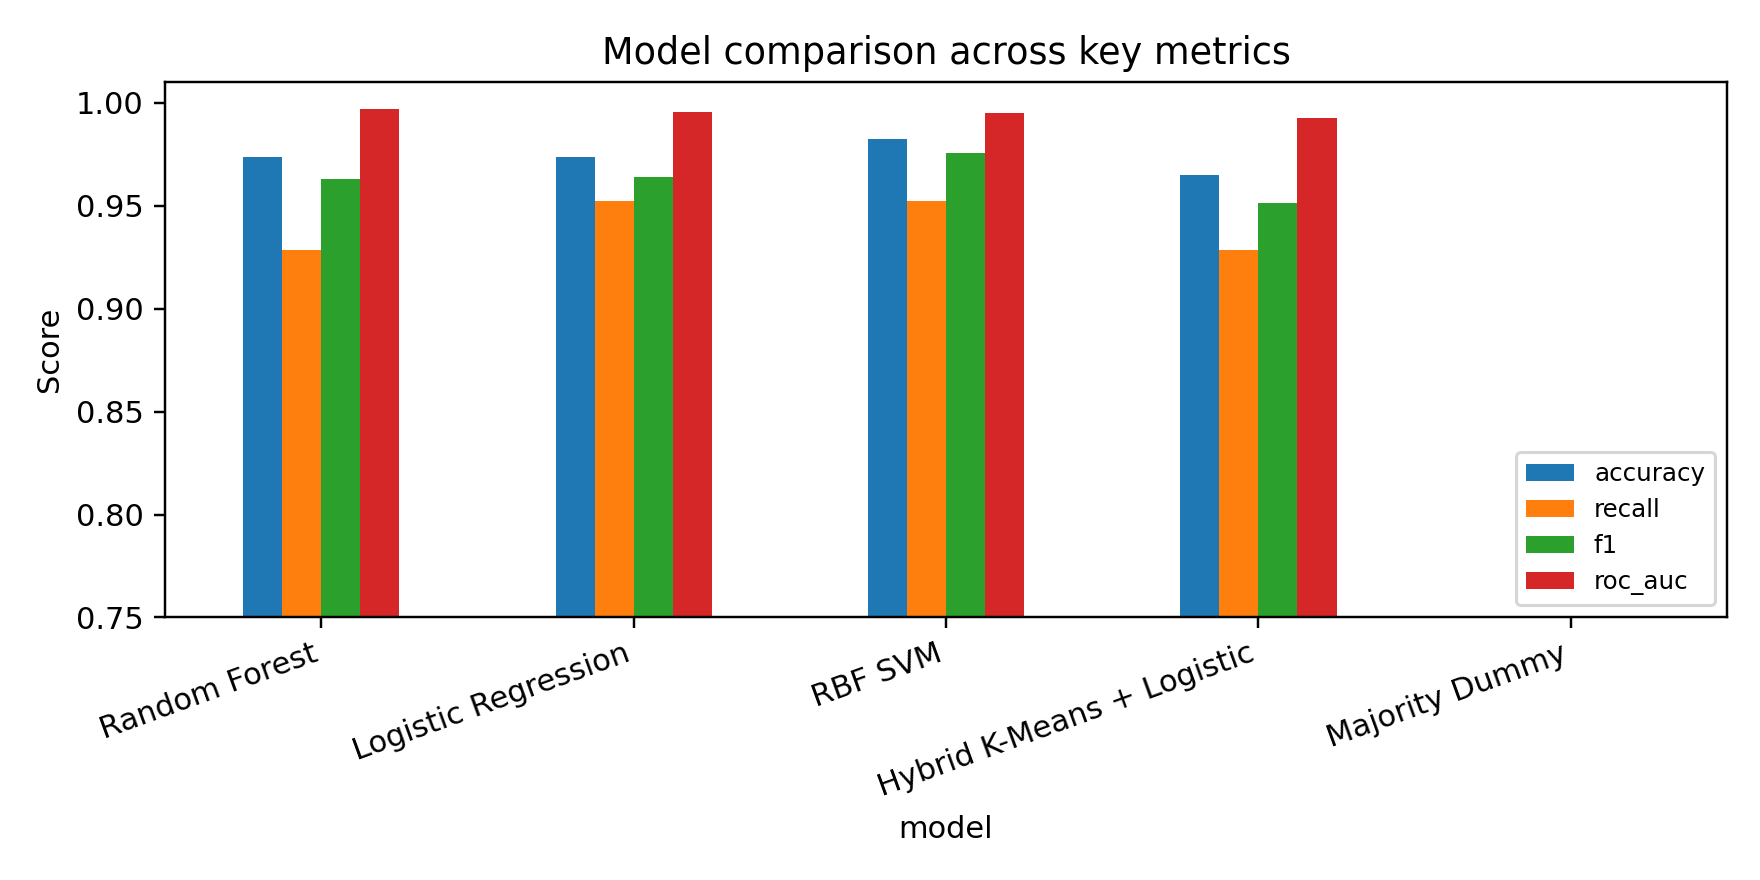
\includegraphics[width=\linewidth]{../outputs/figures/metric_comparison.png}
\caption*{(a) Key metric comparison.}
\end{minipage}
\hfill
\begin{minipage}{0.48\linewidth}
\centering
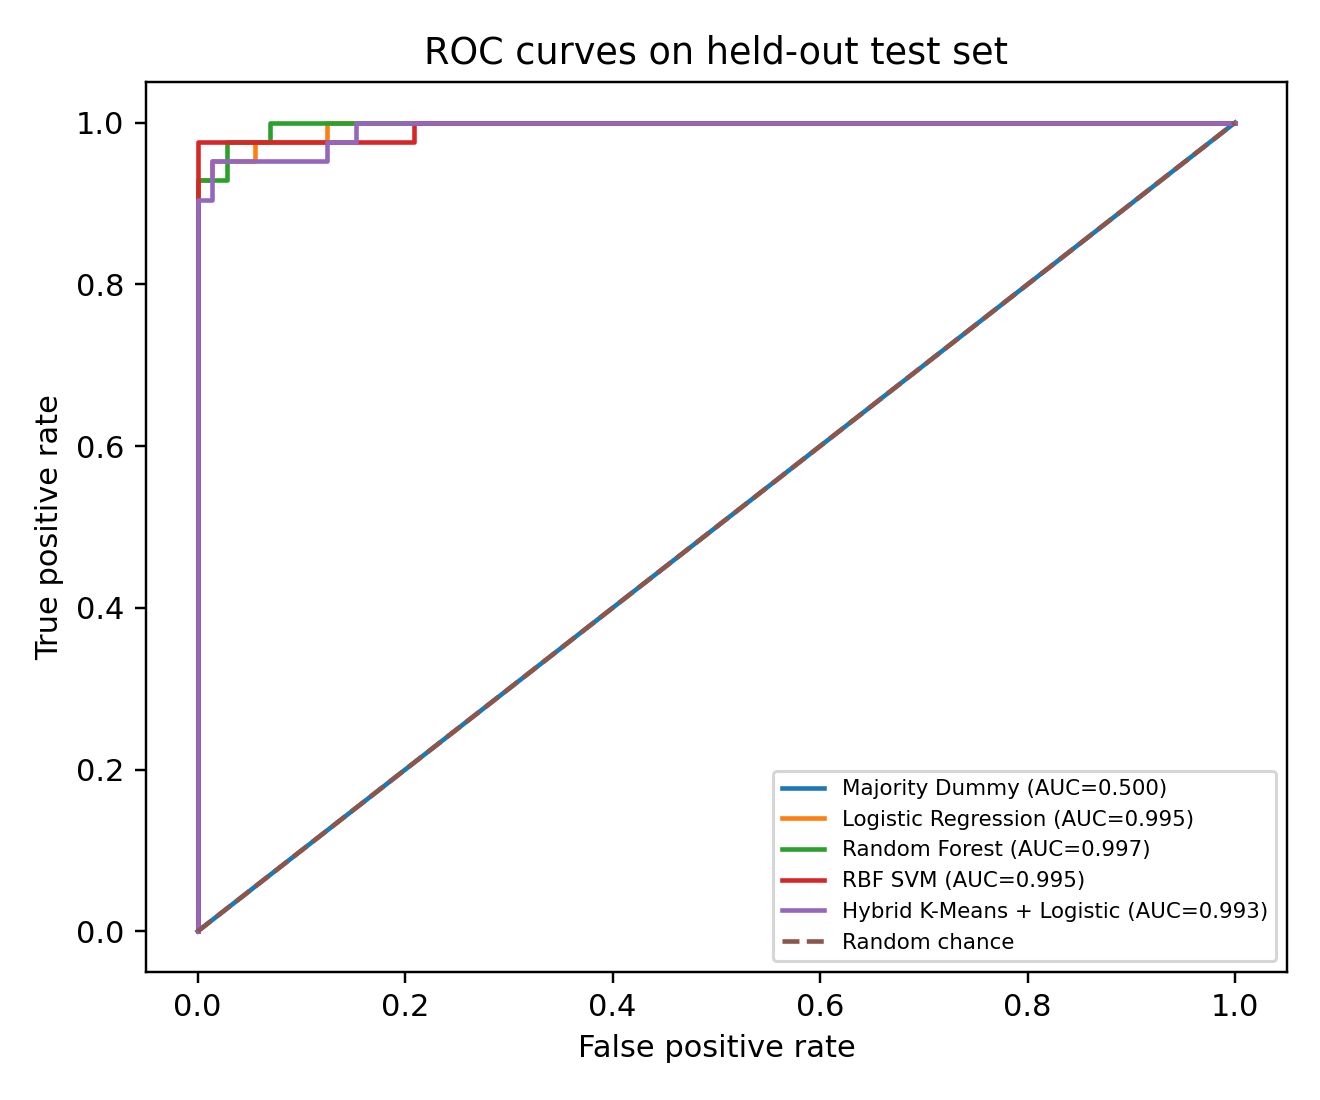
\includegraphics[width=\linewidth]{../outputs/figures/roc_curves.png}
\caption*{(b) ROC curves.}
\end{minipage}
\caption{Supervised baselines and the hybrid model all strongly outperform the dummy baseline. The hybrid model remains
close to the strongest baselines but is slightly weaker on recall and ROC-AUC.}
\label{fig:metrics}
\end{figure}

\subsection{Cross-Validation and Robustness}

To check whether the held-out split was unusual, We also ran 3-fold stratified cross-validation for the main supervised baselines.
Logistic regression and RBF SVM both achieved mean accuracy of 0.9754. RBF SVM had the highest mean ROC-AUC at
0.9951, while logistic regression had 0.9939. Random forest remained strong but had higher recall variation across folds. This
supports the held-out result that the dataset is highly separable and that simpler standardized baselines are already competitive.

\begin{table}[H]
\centering
\caption{Three-fold stratified cross-validation summary for supervised baselines. Values are mean $\pm$ standard deviation.}
\label{tab:cv}
\resizebox{\linewidth}{!}{%
\begin{tabular}{lcccc}
\toprule
Model & Accuracy & Recall & F1 & ROC-AUC \\
\midrule
Logistic Regression & $0.9754 \pm 0.0121$ & $0.9624 \pm 0.0406$ & $0.9668 \pm 0.0164$ & $0.9939 \pm 0.0050$ \\
Random Forest       & $0.9526 \pm 0.0320$ & $0.9154 \pm 0.0975$ & $0.9332 \pm 0.0489$ & $0.9907 \pm 0.0104$ \\
RBF SVM             & $0.9754 \pm 0.0080$ & $0.9671 \pm 0.0325$ & $0.9669 \pm 0.0112$ & $0.9951 \pm 0.0053$ \\
\bottomrule
\end{tabular}%
}
\end{table}

\subsection{Feature Importance and Error Analysis}

Permutation importance was computed for the strongest non-hybrid model by held-out ROC-AUC, which was the random
forest. The most important features are worst concave points, worst area, worst perimeter, worst radius, and worst concavity.
These variables are clinically intuitive because they describe extreme values of cell-nucleus shape and size, which are relevant
to malignancy. The confusion matrices show that all strong models make very few errors, but the remaining errors are mainly
malignant false negatives. This reinforces the importance of threshold analysis in any real clinical setting. A model with
slightly lower overall accuracy may still be preferred if its threshold can be adjusted to reduce false negatives.

\begin{figure}[H]
\centering
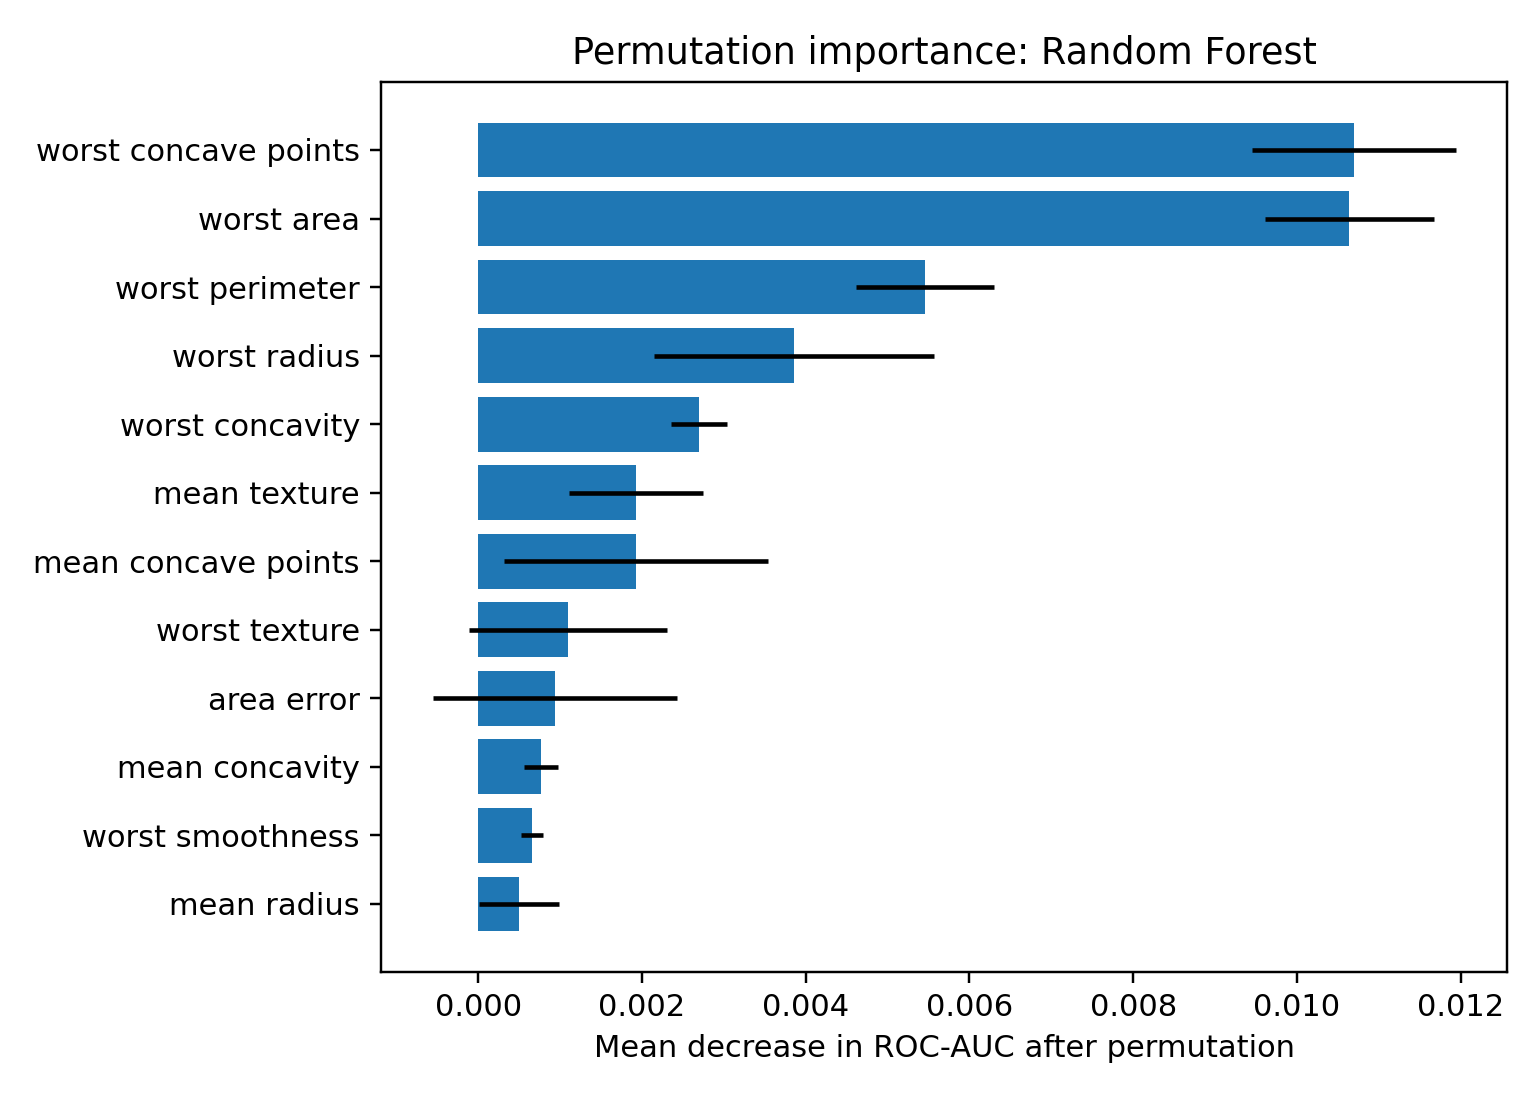
\includegraphics[width=0.76\linewidth]{../outputs/figures/permutation_importance.png}
\caption{Permutation importance for the best ROC-AUC baseline. The strongest signals are worst-case concavity, area,
perimeter, and radius measurements.}
\label{fig:importance}
\end{figure}

\section{Conclusion}

This project developed and evaluated a hybrid unsupervised-supervised diagnosis pipeline for the WDBC dataset. The
strongest held-out accuracy came from the RBF SVM at 98.25\%, and the strongest ROC-AUC came from random forest
at 0.9970. The proposed hybrid K-Means + Logistic model achieved 96.49\% accuracy and 0.9927 ROC-AUC. Therefore,
the main finding is not that unsupervised phenotyping improves predictive performance, but that it provides a compact and
interpretable representation of morphology structure while preserving most of the discriminative signal.

The project has several limitations. The dataset is small, clean, and already highly separable, so performance may
overestimate real-world generalization. The features are precomputed rather than learned directly from medical images. The
K-Means step assumes spherical clusters in standardized Euclidean space, which may be too simple for complex biomedical
subtypes. Future work should test the pipeline on larger multi-site datasets, evaluate calibration and threshold tuning, compare
alternative clustering methods such as Gaussian mixture models or spectral clustering, and validate whether phenotype groups
correspond to medically meaningful subtypes.

\bibliographystyle{plainnat}
\bibliography{references}

\end{document}